\documentclass[10pt,twocolumn,letterpaper]{article}

\usepackage{iccv}
\usepackage{times}
\usepackage{epsfig}
\usepackage{graphicx}
\usepackage{amsmath}
\usepackage{amssymb}
\usepackage{amssymb}
\usepackage{url}
\usepackage{booktabs}
\usepackage{multirow}
\usepackage{subfigure}
\usepackage{lib}
%\usepackage{multirow}
\usepackage{makecell}
%\usepackage{threeparttable}
\usepackage{booktabs}
%\usepackage{stfloats}


%\usepackage[font=small,labelfont=bf,skip=5pt]{caption}

% Include other packages here, before hyperref.

% If you comment hyperref and then uncomment it, you should delete
% egpaper.aux before re-running latex.  (Or just hit 'q' on the first latex
% run, let it finish, and you should be clear).
\usepackage[pagebackref=true,breaklinks=true,letterpaper=true,colorlinks,bookmarks=false]{hyperref}

\iccvfinalcopy % *** Uncomment this line for the final submission

\def\iccvPaperID{1698} % *** Enter the ICCV Paper ID here
\def\httilde{\mbox{\tt\raisebox{-.5ex}{\symbol{126}}}}

% LOCAL COMMANDS
\newcommand{\X}{$\times$\xspace}
\newcommand{\pool}[1]{$\textrm{pool}_{#1}$\xspace}
\newcommand{\conv}[1]{$\textrm{conv}_{#1}$\xspace}
\newcommand{\maxp}[1]{$\textrm{max}_{#1}$\xspace}
\newcommand{\fc}[1]{$\textrm{fc}_{#1}$\xspace}
\newcommand{\vggsixteen}{VGG16\xspace}
\newcommand{\roi}{RoI\xspace}
\newcommand{\Sm}{{\bf S}\xspace}
\newcommand{\Med}{{\bf M}\xspace}
\newcommand{\Lg}{{\bf L}\xspace}
\newcommand{\ZF}{{\bf ZF}\xspace}
\newcommand{\ms}{ms\xspace}
\newcolumntype{x}{>\small c}
\newcolumntype{L}[1]{>{\raggedright\let\newline\\\arraybackslash\hspace{0pt}}m{#1}}
\newcolumntype{C}[1]{>{\centering\let\newline\\\arraybackslash\hspace{0pt}}m{#1}}
\newcolumntype{R}[1]{>{\raggedleft\let\newline\\\arraybackslash\hspace{0pt}}m{#1}}
%%%%%%%%%%%%%%%%

\pagestyle{empty}

\begin{document}

%%%%%%%%% TITLE
\title{Fast R-CNN}

\author{Ross Girshick\\
Microsoft Research\\
{\tt\small rbg@microsoft.com}
}

\maketitle
\thispagestyle{empty}

\begin{abstract}
This paper proposes a Fast Region-based Convolutional Network method \emph{(Fast R-CNN)} for object detection.
Fast R-CNN builds on previous work to efficiently classify object proposals using deep convolutional networks.
Compared to previous work, Fast R-CNN employs several innovations to improve training and testing speed while also increasing detection accuracy.
Fast R-CNN trains the very deep \vggsixteen network 9\X faster than R-CNN, is 213\X faster at test-time, and achieves a higher mAP on PASCAL VOC 2012.
Compared to SPPnet, Fast R-CNN trains \vggsixteen 3\X faster, tests 10\X faster, and is more accurate.
Fast R-CNN is implemented in Python and C++ (using Caffe) and is available under the open-source MIT License at \url{https://github.com/rbgirshick/fast-rcnn}.
\end{abstract}


%\cite{burger2001issues}
%\cite{fader2014open}
%\cite{voorhees1999trec}


%A huge leap forward in artificial intelligence will be achieved when
%machines will be able to answer any question expressed in natural
%language. As such, q

Question answering (QA) has been a long standing research problem in
natural language processing, with the first systems attempting to
answer questions by directly reading
documents \citep{voorhees2000building}. The development of large-scale Knowledge Bases (KBs) such as Freebase  \citep{bollacker2008freebase}
helped organize information into structured forms, prompting recent progress to focus on answering questions by converting them into logical forms that can be used to query such databases \citep{berant2013semantic,kwiatkowski-EtAl:2013:EMNLP,fader2014open}.

Unfortunately, KBs have intrinsic limitations such as their inevitable incompleteness and fixed schemas that cannot support all varieties of answers.
%
Since information extraction (IE) \citep{craven2000learning}, intended to
fill in missing information in KBs, is neither accurate nor
reliable enough, collections of raw textual resources and
documents such as Wikipedia will always contain more information.
%than KBs.
%
As a result, even if KBs can be satisfactory for closed-domain problems, they are unlikely
to scale up to answer general questions on any
topic.
%
Starting from this observation,
%here we propose  to study the problem
in this work we study the problem
of answering by directly reading documents.


Retrieving answers directly from text is harder than
from KBs because information is far less structured, is
indirectly and ambiguously expressed, and is usually scattered across multiple documents.
%
%This explains why, when a satisfactory KB is
%available -- which is typically only the case in closed domains --
%using it instead of raw text is preferred. %, because performance is better.
%
This explains why using a satisfactory KB---typically only available in closed domains---is preferred over raw text.
%
We postulate that before trying to provide answers that are not in
KBs, document-based QA systems should first reach KB-based systems'
performance in such closed domains, where clear comparison and
evaluation is possible.
%
To this end, this paper introduces {\sc WikiMovies}, a new
analysis tool that allows for measuring the performance of %loss induced on
QA systems when the knowledge source is switched from a KB to unstructured documents.
%
{\sc WikiMovies} contains $\sim$100k questions in the movie domain, and was designed
to be answerable by using either a perfect KB
(based on OMDb\footnote{\url{http://www.omdbapi.com}}), Wikipedia pages or an imperfect KB obtained through
running %a standard IE pipeline on those pages.
an engineered IE pipeline on those pages.

To bridge the gap between using a KB and reading documents directly,
we still lack appropriate machine learning algorithms. In this
work we propose the Key-Value Memory Network (KV-MemNN), a new neural network
architecture that generalizes the original Memory Network
\citep{sukhbaatar2015end} and can work with either knowledge source.
%
The KV-MemNN performs QA by first storing facts in a key-value
structured memory before reasoning on them in order to predict an
answer. The memory is designed so that the model learns to use keys to
address relevant memories with respect to the question, whose corresponding values are subsequently returned.
%
This structure allows the model to encode prior knowledge for the considered task
and to leverage possibly complex transforms between keys and values,
while still being trained using standard backpropagation via
stochastic gradient descent.

Our experiments on {\sc WikiMovies} indicate that, thanks to its key-value memory,
the KV-MemNN consistently outperforms the
original Memory Network, and reduces the gap between answering from a human-annotated KB,
from an automatically extracted KB or from directly reading Wikipedia.
%
We confirm our findings on  {\sc WikiQA} \citep{yang2015wikiqa},
another Wikipedia-based QA benchmark where no KB is available,
where we demonstrate that KV-MemNN can reach state-of-the-art results---surpassing
the most recent attention-based neural network models.

\begin{figure*}
\centering
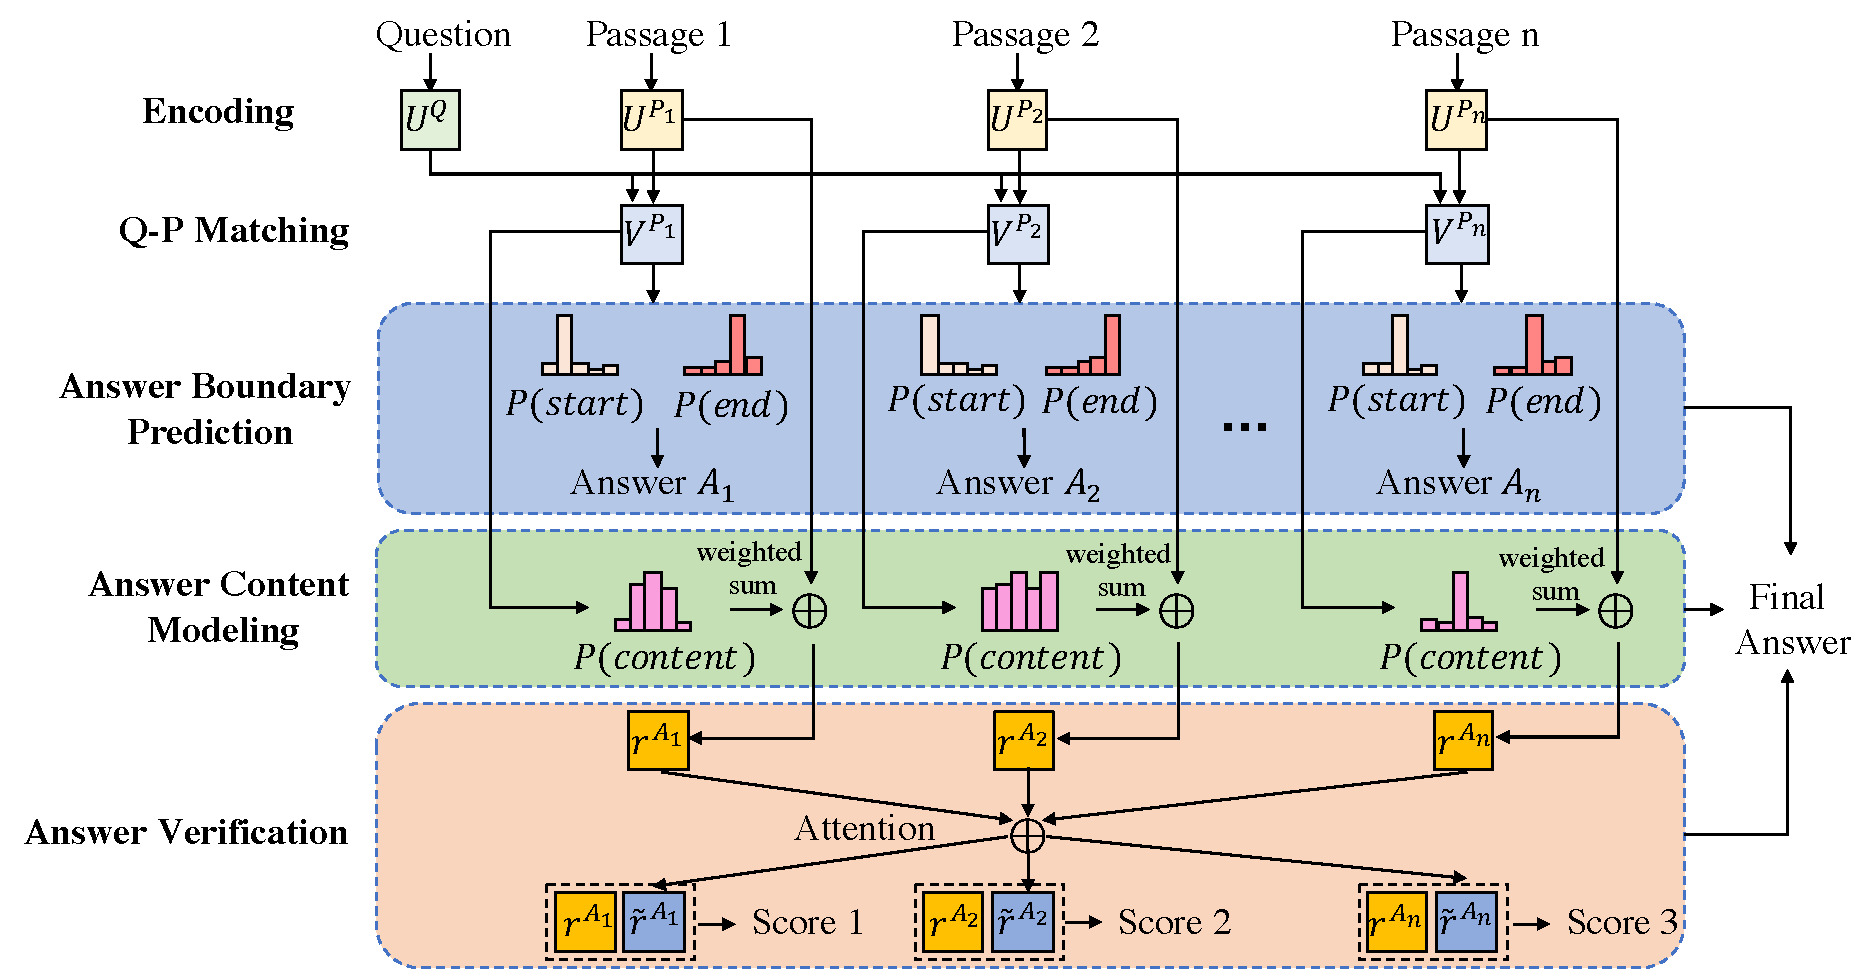
\includegraphics[width=0.85\textwidth]{architecture}
\caption{The overall architecture of our proposed network. The network
contains layers of symmetric convolution (encoder) and deconvolution (decoder).
Skip shortcuts are connected every a few (in our experiments, two) layers from
convolutional feature maps to their mirrored deconvolutional feature maps.
The response from a convolutional layer is directly propagated to the corresponding
mirrored deconvolutional layer, both forwardly and backwardly.}
\label{fig1}
\end{figure*}

\section{Very deep convolutional auto-encoder for image restoration}
\label{sec:main}

The proposed framework mainly contains a chain of convolutional layers and symmetric
deconvolutional layers, as shown in Figure \ref{fig1}. Skip connections are connected
symmetrically from convolutional layers to deconvolutional layers. We term our method
``RED-Net''---very deep Residual Encoder-Decoder Networks.


\subsection{Architecture}

The framework is fully convolutional (and deconvolutional.  Deconvolution is essentially unsampling convolution). Rectification layers are added
after each convolution and deconvolution. For low-level image restoration problems, we
use neither pooling nor unpooling in the network as usually pooling discards useful image
details that are essential for these tasks. It is worth mentioning that since the convolutional
and deconvolutional layers are symmetric, the network is essentially pixel-wise prediction,
thus the size of input image can be arbitrary. The input and output of the network are images
of the same size $w\times h\times c$, where $w$, $h$ and $c$ are width, height and number of channels.

Our main idea is that the convolutional layers act as a feature extractor, which preserve the
primary components of objects in the image and meanwhile eliminating the corruptions.
After forwarding through the convolutional layers, the corrupted input  image is converted into
a ``clean" one. The subtle details of the image contents may be lost during this process.
The deconvolutional layers are then combined to recover the details of image contents.
The output of the deconvolutional layers is the recovered clean version of the input image.
Moreover, we add skip connections  from a convolutional layer to its corresponding
mirrored deconvolutional layer. The passed convolutional feature maps are summed to the
deconvolutional feature maps element-wise, and passed to the next layer after rectification.
Deriving from the above architecture, we have used two networksvin our experiments, which are of 20 layers
 and 30 layers
respectively, for image denoising, image super-resolution, JPEG deblocking and image inpainting.



\subsection{Deconvolution decoder}

Architectures combining layers of convolution and deconvolution~\cite{DBLP:conf/iccv/NohHH15,
hong2015decoupled} have been proposed for semantic segmentation recently. In contrast to
convolutional layers, in which multiple input activations within a filter window are fused
to output a single activation, deconvolutional layers associate a single input activation with
multiple outputs. Deconvolution is usually used as {\em learnable up-sampling layers}.

 In our network,
the convolutional layers successively down-sample the input image content into a  small
size abstraction. Deconvolutional layers then up-sample the abstraction back into its original resolution.

Besides the use of skip connections, a main difference between our model and
~\cite{DBLP:conf/iccv/NohHH15,hong2015decoupled} is that our network is fully convolutional and
deconvolutional, i.e., without pooling and un-pooling. The reason is that for low-level image restoration,
the aim is to eliminate low level corruption while preserving image details instead of learning
image abstractions. Different from high-level applications such as segmentation or recognition,
pooling typically eliminates the abundant image details and can deteriorate restoration performance.



One can simply replace deconvolution with convolution, which results in an architecture that is
very similar to recently proposed very deep fully convolutional neural networks
~\cite{DBLP:conf/cvpr/LongSD15,DBLP:journals/pami/DongLHT16}. However, there exist essential
differences between a fully convolution model and our model. Take image denoising as an example.
We compare the 5-layer and 10-layer fully convolutional network with our network
(combining convolution and deconvolution, but without skip connection). For fully convolutional
networks, we use padding or up-sampling the input to make the input and output be of the same size.
For our network, the first 5 layers are convolutional and the second 5 layers are deconvolutional.
All the other parameters for training are identical, i.e., trained with SGD and learning rate of
$10^{-6}$, noise level $\sigma=70$. The Peak Signal-to-Noise Ratio (PSNR) on the validation set
is reported, which shows that using deconvolution works better than the fully convolutional
counterpart, as shown in Figure \ref{fig2}.


Furthermore, in Figure \ref{fig3}, we visualize some results that are outputs of layer 2, 5, 8 and 10
from the 10-layer fully convolutional network and ours. In the fully convolution case, the noise
is eliminated step by step, i.e., the noise level is reduced after each layer. During this process,
the details of the image content may be lost. Nevertheless, in our network, convolution  preserves
the primary image content. Then deconvolution is used to compensate the details.


\begin{figure}[htb!]
\centering
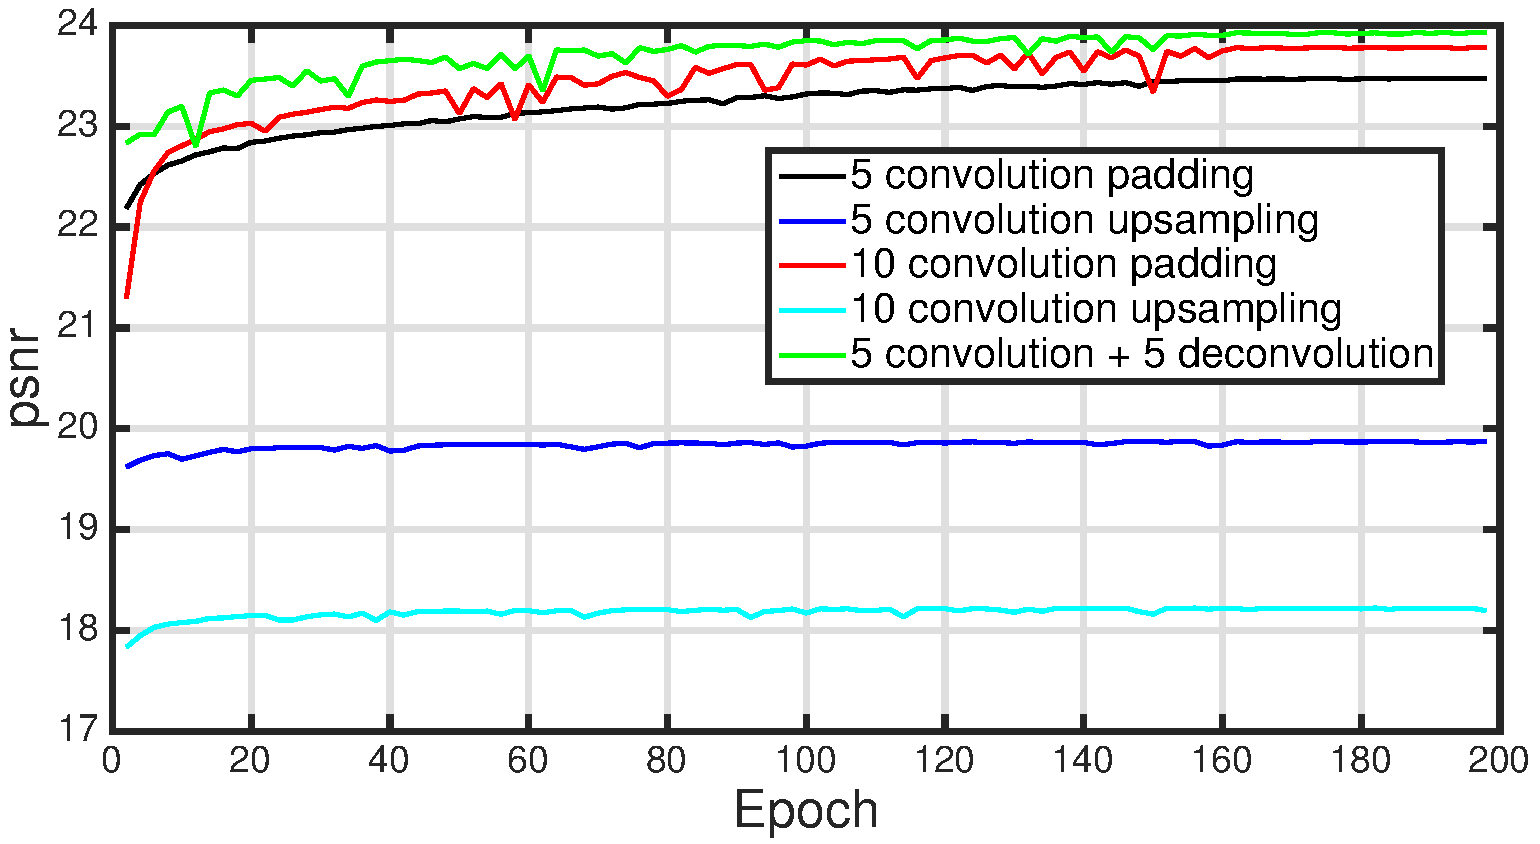
\includegraphics[width=0.48\textwidth]{conv-vs-decv}
\caption{ PSNR  values  on the validation set during training. Our model  exhibits better PSNR
than the compared ones upon convergence.}
\label{fig2}
\end{figure}



\begin{figure}[htb!]
\centering
\subfigure[]{ 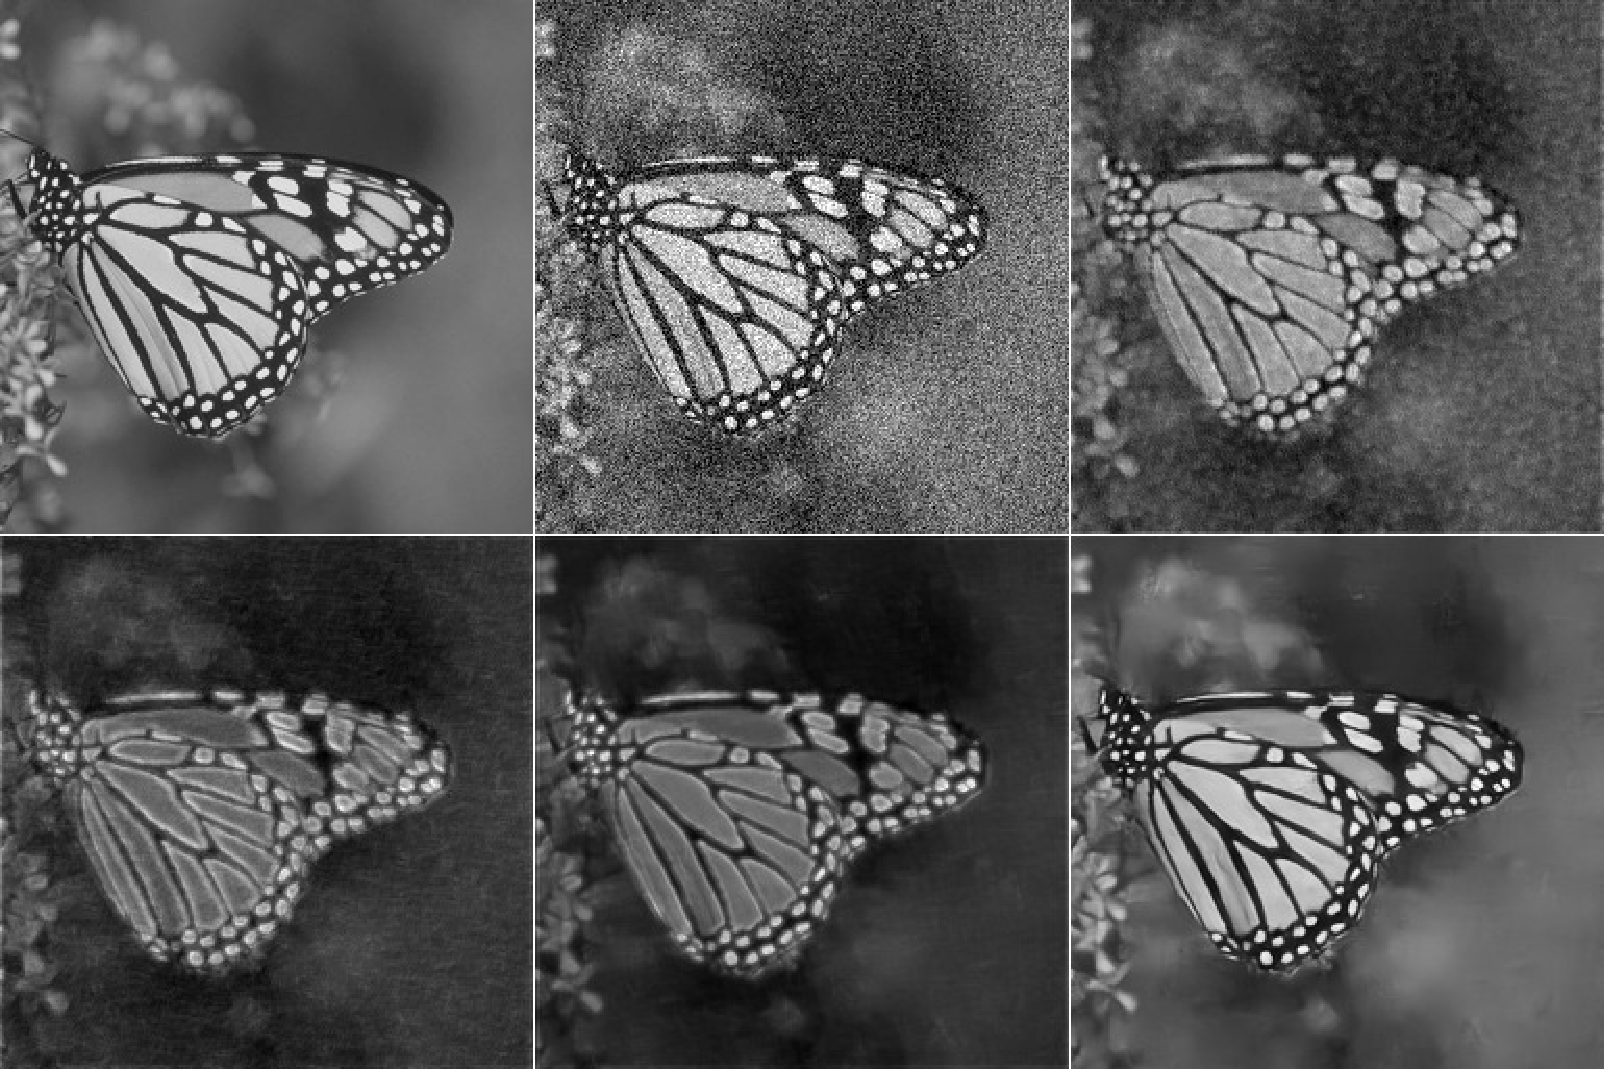
\includegraphics[width=0.48\textwidth]{show-denoising-conv} }
\subfigure[]{ 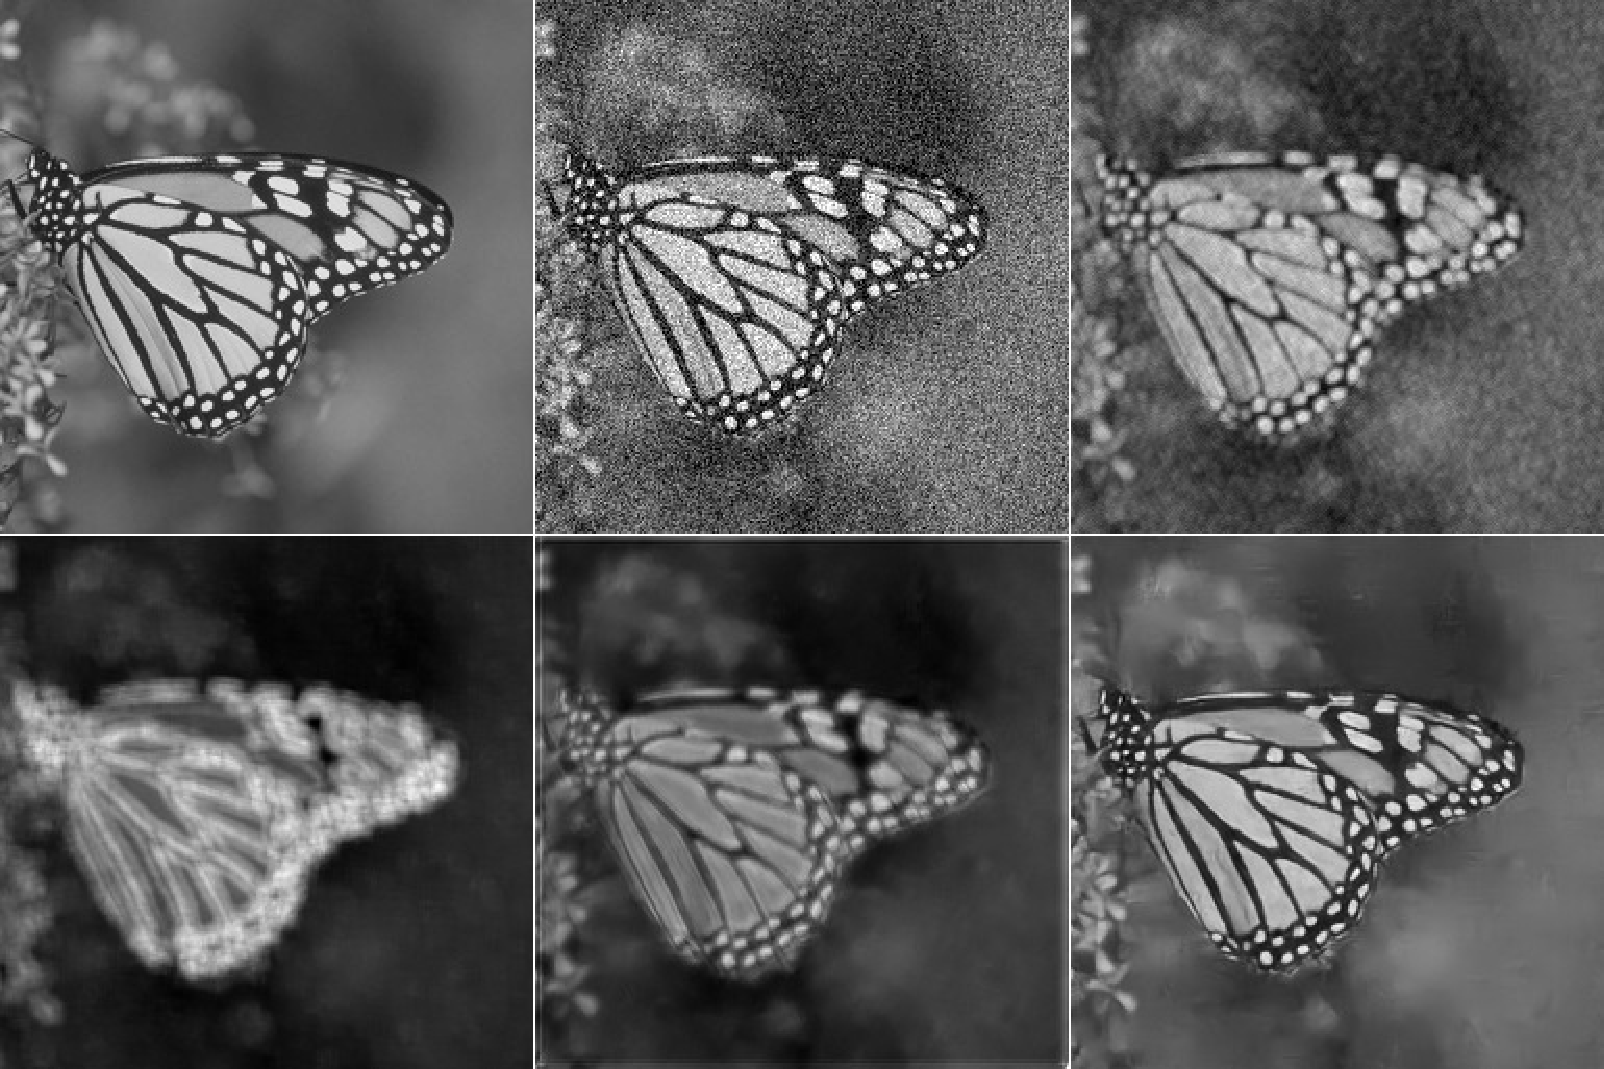
\includegraphics[width=0.48\textwidth]{show-denoising-decv} }
\caption{ (a) Visualization of the 10-layer fully convolutional network. The images from
top-left to bottom-right are: clean image, noisy image, output of conv-2, output of conv-5,
output of conv-8 and output of conv-10, where ``conv-$i$" stands for the $i$-th convolutional layer;
(b) Visualization of the 10-layer convolutional and deconvolutional network. The images from
top-left to bottom-right are: clean image, noisy image, output of conv-2, output of conv-5,
output of deconv-3 and output of deconv-5, where ``deconv-$i$" stands for the $i$-th deconvolutional layer.}
\label{fig3}
\end{figure}




\subsection{Skip connections}

An intuitive question is that, is a network with deconvolution able to recover image details from
the image abstraction only? We find that in shallow networks with only a few layers
of convolution layers, deconvolution is able to recover the details. However, when the
network goes deeper or using operations such as max pooling, even with deconvolution layers, it does not work
that well, possibly because too much details are already lost in the convolution and pooling.


The second question is that, when our network goes deeper, does it achieve performance gain?
We observe that deeper networks in image restoration tasks tend to easily suffer from
performance degradation. The reason may be two folds. First of all, with more layers of
convolution, a significant amount of image details could be lost or corrupted. Given only the image abstraction,
recovering its details is an under-determined problem. Secondly, in terms of optimization,
deep networks often suffer from gradients vanishing and become much harder to train---a problem
that is well addressed in the literature of neural networks.


To address the above two problems, inspired by highway networks \cite{DBLP:journals/corr/SrivastavaGS15}
and deep residual networks \cite{DBLP:journals/corr/HeZRS15}, we add skip connections between
two corresponding convolutional and deconvolutional layers as shown in Figure \ref{fig1}.
A building block is shown in Figure \ref{fig4}. There are two reasons for using such connections.
First, when the network goes deeper, as mentioned above, image details can be lost, making deconvolution
weaker in recovering them. However, the feature maps passed by skip connections carry much image detail,
which helps deconvolution to recover an improved clean version of the image. Second, the skip connections also achieve
benefits on back-propagating the gradient to bottom layers, which makes training deeper network much
easier as observed in \cite{DBLP:journals/corr/SrivastavaGS15} and \cite{DBLP:journals/corr/HeZRS15}.

Note that our skip layer connections are very different from the ones proposed in
\cite{DBLP:journals/corr/SrivastavaGS15} and \cite{DBLP:journals/corr/HeZRS15}, where the only concern
is on the optimization side. In our case, we want to pass information of the convolutional feature maps
to the corresponding deconvolutional layers. The very deep highway networks
\cite{DBLP:journals/corr/SrivastavaGS15} are essentially feedforward long short-term memory (LSTMs)
with forget gates, and the CNN layers of deep residual network \cite{DBLP:journals/corr/HeZRS15}
are feedforward LSTMs without gates. Note that our networks are in general not in the format of
standard feedforward LSTMs.

\begin{figure}[htb!]
\centering
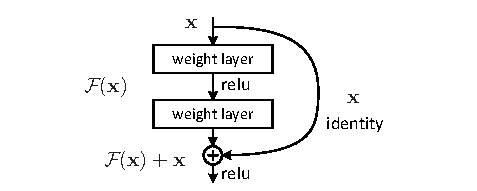
\includegraphics[width=0.48\textwidth]{block}
\caption{An example of a building block in the proposed framework. The rectangle in solid and
dotted lines denote convolution and deconvolution respectively. $\oplus$ denotes element-wise sum of feature maps.}
\label{fig4}
\end{figure}

Instead of directly learning the mappings from the input $X$ to the output $Y$, we would like the network
to fit the residual~\cite{DBLP:journals/corr/HeZRS15} of the problem, which is denoted as $\mathcal{F}(X)=Y-X$.
Such a learning strategy is applied to inner blocks of the encoding-decoding network to make training more
effective. Skip connections are passed every two convolutional layers to their mirrored deconvolutional
layers. Other configurations are possible and our experiments show that this configuration already works
very well. Using such shortcuts makes the network easier to be trained and gains restoration performance
by increasing the network depth.




\subsection{Training}

In general, there are three types of layers in our network: convolution, deconvolution
and element-wise sum. Each layer is followed by a Rectified Linear Unit (ReLU)
~\cite{DBLP:conf/icml/NairH10}. Let $X$ be the input, the convolutional and
deconvolutional layers are expressed as:
\begin{equation}
F(X) = \max(0,W_k * X + B_k),
\end{equation}
where $W_k$ and $B_k$ represent the filters and biases, and $*$ denotes either
convolution or deconvolution operation for the convenience of formulation.
For element-wise sum layer, the output is the element-wise sum of two inputs
of the same size, followed by the ReLU activation:
\begin{equation}
F(X_1,X_2) = \max(0, X_1 + X_2)
\end{equation}

Learning the end-to-end mapping from corrupted images to clean images needs to
estimate the weights $\Theta$ represented by the convolutional and deconvolutional
kernels. Specifically, given a collection of $N$ training sample pairs $\{X^i,Y^i\}$,
where $X^i$ is a noisy image and $Y^i$ is the clean version as the groundtruth.
We minimize the following Mean Squared Error (MSE):
\begin{equation}
  \mathcal{L}(\Theta) = \frac{1}{N}\sum_{i=1}^{N}\|\mathcal{F}(X^i;\Theta)-Y^i\|_F^2.
\label{eq1}
\end{equation}

Traditionally, a  network can learn the mapping from the corrupted image to the clean version
directly. However, our network learns for the additive corruption from the input since there
is a skip connection between the input and the output of the network.
%
%
%
We found that optimizing for the corruption converges better than
optimizing for the clean image. In the extreme case, if the input is a clean image, it would be easier
to push the network to be zero mapping (learning the corruption) than to fit an identity
mapping (learning the clean image) with a stack of nonlinear layers.

We implement and train our network using Caffe~\cite{jia2014caffe}. Empirically, we find
that using Adam~\cite{DBLP:journals/corr/KingmaB14} with base learning rate of $10^{-4}$ for
training converges faster than traditional stochastic gradient descent (SGD). The base
learning rate for all layers are the same, different from ~\cite{DBLP:journals/pami/DongLHT16,
DBLP:conf/nips/JainS08}, in which a smaller learning rate is set for the last layer.
This  is not necessary in our network. Specifically, gradients with respect to the
parameters of $i$th layer is firstly computed as:
\begin{equation}
g = \nabla_{\theta_i}\mathcal{L}(\theta_i).
\end{equation}
Then, the two momentum vectors are computed as:
\begin{equation}
m = \beta_1m + (1 - \beta_1)g,\quad v = \beta_2v + (1-\beta_2)g^2.
\end{equation}
The update rule is:
\begin{equation}
\alpha = \alpha\sqrt{1-\beta_2^t}/(1-\beta_1^t), \quad \theta_i=\theta_i-\alpha m/(\sqrt{v}+\epsilon).
\end{equation}
$\beta_1$, $\beta_2$ and $\epsilon$ are set as the recommended values in~\cite{DBLP:journals/corr/KingmaB14}.

300 images from the Berkeley Segmentation Dataset (BSD)~\cite{MartinFTM01} are used to
generate image patches as the training set for each image restoration task.
%
%
%




\subsection{Testing}

Although trained on local patches, our network can perform restoration on images of arbitrary sizes.
Given a testing image, one can simply go forward through the network, which is already able to
 outperform existing methods. To achieve even better results, we propose
to process a corrupted image on multiple orientations. Different from segmentation, the
filter kernels in our network only eliminate the corruptions, which is usually not sensitive
to the orientation of image contents in low level restoration tasks. Therefore, we can rotate
and mirror flip the kernels and perform forward multiple times, and then average the output to
achieve an ensemble of multiple tests. We see that this can lead to slightly better performance.

\section{Main results}

\begin{table*}[t!]
\centering
\renewcommand{\arraystretch}{1.2}
\renewcommand{\tabcolsep}{1.2mm}
\resizebox{\linewidth}{!}{
  \begin{tabular}{@{}L{2.5cm}|L{1.2cm}|r*{19}{x}|x@{}}
method & train set & aero      & bike      & bird      & boat      & bottle     & bus        & car        & cat        & chair      & cow        & table      & dog        & horse      & mbike      & persn     & plant      & sheep      & sofa       & train      & tv         & mAP       \\
\hline
SPPnet BB \cite{he2014spp}$^\dagger$ &
07 $\setminus$ diff &
73.9 &
72.3 &
62.5 &
51.5 &
44.4 &
74.4 &
73.0 &
74.4 &
42.3 &
73.6 &
57.7 &
70.3 &
74.6 &
74.3 &
54.2 &
34.0 &
56.4 &
56.4 &
67.9 &
73.5 &
63.1 \\
R-CNN BB \cite{rcnn-pami} &
07 &
73.4 &
77.0 &
63.4 &
45.4 &
\bf{44.6} &
75.1 &
78.1 &
79.8 &
40.5 &
73.7 &
62.2 &
79.4 &
78.1 &
73.1 &
64.2 &
\bf{35.6} &
66.8 &
67.2 &
70.4 &
\bf{71.1} &
66.0 \\
\hline
FRCN [ours] &
07 &
74.5 &
78.3 &
69.2 &
53.2 &
36.6 &
77.3 &
78.2 &
82.0 &
40.7 &
72.7 &
67.9 &
79.6 &
79.2 &
73.0 &
69.0 &
30.1 &
65.4 &
70.2 &
75.8 &
65.8 &
66.9 \\
FRCN [ours] &
07 $\setminus$ diff &
74.6 &
\bf{79.0} &
68.6 &
57.0 &
39.3 &
79.5 &
\bf{78.6} &
81.9 &
\bf{48.0} &
74.0 &
67.4 &
80.5 &
80.7 &
74.1 &
69.6 &
31.8 &
67.1 &
68.4 &
75.3 &
65.5 &
68.1 \\
FRCN [ours] &
07+12 &
\bf{77.0} &
78.1 &
\bf{69.3} &
\bf{59.4} &
38.3 &
\bf{81.6} &
\bf{78.6} &
\bf{86.7} &
42.8 &
\bf{78.8} &
\bf{68.9} &
\bf{84.7} &
\bf{82.0} &
\bf{76.6} &
\bf{69.9} &
31.8 &
\bf{70.1} &
\bf{74.8} &
\bf{80.4} &
70.4 &
\bf{70.0} \\
\end{tabular}
}
\vspace{0.05em}
\caption{{\bf VOC 2007 test} detection average precision (\%). All methods use \vggsixteen. Training set key: {\bf 07}: VOC07 trainval, {\bf 07 $\setminus$ diff}: {\bf 07} without ``difficult'' examples, {\bf 07+12}: union of {\bf 07} and VOC12 trainval.
$^\dagger$SPPnet results were prepared by the authors of \cite{he2014spp}.}
\tablelabel{voc2007}
\end{table*}

\begin{table*}[t!]
\centering
\renewcommand{\arraystretch}{1.2}
\renewcommand{\tabcolsep}{1.2mm}
\resizebox{\linewidth}{!}{
\begin{tabular}{@{}L{2.5cm}|L{1.2cm}|r*{19}{x}|x@{}}
method & train set & aero      & bike      & bird      & boat      & bottle     & bus        & car        & cat        & chair      & cow        & table      & dog        & horse      & mbike      & persn     & plant      & sheep      & sofa       & train      & tv         & mAP       \\
\hline
BabyLearning &
Prop. &
77.7 &
73.8 &
62.3 &
48.8 &
45.4 &
67.3 &
67.0 &
80.3 &
41.3 &
70.8 &
49.7 &
79.5 &
74.7 &
78.6 &
64.5 &
36.0 &
69.9 &
55.7 &
70.4 &
61.7 &
63.8 \\
R-CNN BB \cite{rcnn-pami} &
12 &
79.3 &
72.4 &
63.1 &
44.0 &
44.4 &
64.6 &
66.3 &
84.9 &
38.8 &
67.3 &
48.4 &
82.3 &
75.0 &
76.7 &
65.7 &
35.8 &
66.2 &
54.8 &
69.1 &
58.8 &
62.9 \\
SegDeepM &
12+seg &
\bf{82.3} &
75.2 &
67.1 &
50.7 &
\bf{49.8} &
71.1 &
69.6 &
88.2 &
42.5 &
71.2 &
50.0 &
85.7 &
76.6 &
81.8 &
69.3 &
\bf{41.5} &
\bf{71.9} &
62.2 &
73.2 &
\bf{64.6} &
67.2 \\
\hline
FRCN [ours] &
12 &
80.1 &
74.4 &
67.7 &
49.4 &
41.4 &
74.2 &
68.8 &
87.8 &
41.9 &
70.1 &
50.2 &
86.1 &
77.3 &
81.1 &
70.4 &
33.3 &
67.0 &
63.3 &
77.2 &
60.0 &
66.1 \\
FRCN [ours] &
07++12 &
82.0 &
\bf{77.8} &
\bf{71.6} &
\bf{55.3} &
42.4 &
\bf{77.3} &
\bf{71.7} &
\bf{89.3} &
\bf{44.5} &
\bf{72.1} &
\bf{53.7} &
\bf{87.7} &
\bf{80.0} &
\bf{82.5} &
\bf{72.7} &
36.6 &
68.7 &
\bf{65.4} &
\bf{81.1} &
62.7 &
\bf{68.8} \\
\end{tabular}
}
\vspace{0.05em}
\caption{{\bf VOC 2010 test} detection average precision (\%).
BabyLearning uses a network based on \cite{Lin2014NiN}.
All other methods use \vggsixteen. Training set key: {\bf 12}: VOC12 trainval, {\bf Prop.}: proprietary dataset, {\bf 12+seg}: {\bf 12} with segmentation annotations, {\bf 07++12}: union of VOC07 trainval, VOC07 test, and VOC12 trainval.
%Results:
%$^\dagger$\url{http://host.robots.ox.ac.uk:8080/anonymous/UKA8XB.html},
%$^\dagger$\url{http://goo.gl/f1vtls},
%$^\ddagger$\url{http://host.robots.ox.ac.uk:8080/anonymous/DGTVGW.html}
%$^\ddagger$\url{http://goo.gl/kyZcnW}
}
\tablelabel{voc2010}
\end{table*}

\begin{table*}[t!]
\centering
\renewcommand{\arraystretch}{1.2}
\renewcommand{\tabcolsep}{1.2mm}
\resizebox{\linewidth}{!}{
  \begin{tabular}{@{}L{2.5cm}|L{1.2cm}|r*{19}{x}|x@{}}
method & train set & aero      & bike      & bird      & boat      & bottle     & bus        & car        & cat        & chair      & cow        & table      & dog        & horse      & mbike      & persn     & plant      & sheep      & sofa       & train      & tv         & mAP       \\
\hline
BabyLearning &
Prop. &
78.0 &
74.2 &
61.3 &
45.7 &
42.7 &
68.2 &
66.8 &
80.2 &
40.6 &
70.0 &
49.8 &
79.0 &
74.5 &
77.9 &
64.0 &
35.3 &
67.9 &
55.7 &
68.7 &
62.6 &
63.2 \\
NUS\_NIN\_c2000 &
Unk. &
80.2 &
73.8 &
61.9 &
43.7 &
\bf{43.0} &
70.3 &
67.6 &
80.7 &
41.9 &
69.7 &
51.7 &
78.2 &
75.2 &
76.9 &
65.1 &
\bf{38.6} &
\bf{68.3} &
58.0 &
68.7 &
63.3 &
63.8 \\
R-CNN BB \cite{rcnn-pami} &
12 &
79.6 &
72.7 &
61.9 &
41.2 &
41.9 &
65.9 &
66.4 &
84.6 &
38.5 &
67.2 &
46.7 &
82.0 &
74.8 &
76.0 &
65.2 &
35.6 &
65.4 &
54.2 &
67.4 &
60.3 &
62.4 \\
\hline
FRCN [ours] &
12 &
80.3 &
74.7 &
66.9 &
46.9 &
37.7 &
73.9 &
68.6 &
87.7 &
41.7 &
71.1 &
51.1 &
86.0 &
77.8 &
79.8 &
69.8 &
32.1 &
65.5 &
63.8 &
76.4 &
61.7 &
65.7 \\
FRCN [ours] &
07++12 &
\bf{82.3} &
\bf{78.4} &
\bf{70.8} &
\bf{52.3} &
38.7 &
\bf{77.8} &
\bf{71.6} &
\bf{89.3} &
\bf{44.2} &
\bf{73.0} &
\bf{55.0} &
\bf{87.5} &
\bf{80.5} &
\bf{80.8} &
\bf{72.0} &
35.1 &
\bf{68.3} &
\bf{65.7} &
\bf{80.4} &
\bf{64.2} &
\bf{68.4} \\
\end{tabular}
}
\vspace{0.05em}
\caption{{\bf VOC 2012 test} detection average precision (\%).
BabyLearning and NUS\_NIN\_c2000 use networks based on \cite{Lin2014NiN}.
All other methods use \vggsixteen. Training set key: see \tableref{voc2010}, {\bf Unk.}: unknown.
%Results:
%$^\dagger$\url{http://host.robots.ox.ac.uk:8080/anonymous/QMSIIY.html},
%$^\ddagger$\url{http://host.robots.ox.ac.uk:8080/anonymous/DCSBZY.html}
%$^\dagger$\url{http://goo.gl/weNq2Z},
%$^\ddagger$\url{http://goo.gl/o1tZ10}
}
\tablelabel{voc2012}
\end{table*}



Three main results support this paper's contributions:
\begin{enumerate}
  \itemsep0em
  \item State-of-the-art mAP on VOC07, 2010, and 2012
  \item Fast training and testing compared to R-CNN, SPPnet
  \item Fine-tuning conv layers in \vggsixteen improves mAP
\end{enumerate}

\subsection{Experimental setup}
\seclabel{setup}
Our experiments use three pre-trained ImageNet models that are available online.\footnote{\url{https://github.com/BVLC/caffe/wiki/Model-Zoo}}
The first is the CaffeNet (essentially AlexNet \cite{krizhevsky2012imagenet}) from R-CNN \cite{girshick2014rcnn}.
We alternatively refer to this CaffeNet as model \Sm, for ``small.''
The second network is VGG\_CNN\_M\_1024 from \cite{Chatfield14}, which has the same depth as \Sm, but is wider.
We call this network model \Med, for ``medium.''
The final network is the very deep \vggsixteen model from \cite{simonyan2015verydeep}.
Since this model is the largest, we call it model \Lg.
In this section, all experiments use \emph{single-scale} training and testing ($s = 600$; see \secref{scale} for details).

\subsection{VOC 2010 and 2012 results}
On these datasets, we compare Fast R-CNN (\emph{FRCN}, for short) against the top methods on the \texttt{comp4} (outside data) track from the public leaderboard (\tableref{voc2010}, \tableref{voc2012}).\footnote{\url{http://host.robots.ox.ac.uk:8080/leaderboard} (accessed April 18, 2015)}
For the NUS\_NIN\_c2000 and BabyLearning methods, there are no associated publications at this time and we could not find exact information on the ConvNet architectures used; they are variants of the Network-in-Network design \cite{Lin2014NiN}.
All other methods are initialized from the same pre-trained \vggsixteen network.
%We show results when training on the VOC12 trainval image set as well as an augmented dataset that includes all annotated images in VOC07.

Fast R-CNN achieves the top result on VOC12 with a mAP of 65.7\% (and 68.4\% with extra data).
It is also two orders of magnitude faster than the other methods, which are all based on the ``slow'' R-CNN pipeline.
On VOC10, SegDeepM \cite{Zhu2015segDeepM} achieves a higher mAP than Fast R-CNN (67.2\% vs. 66.1\%).
SegDeepM is trained on VOC12 trainval plus segmentation annotations; it is designed to boost R-CNN accuracy by using a Markov random field to reason over R-CNN detections and segmentations from the O$_2$P \cite{o2p} semantic-segmentation method.
Fast R-CNN can be swapped into SegDeepM in place of R-CNN, which may lead to better results.
When using the enlarged 07++12 training set (see \tableref{voc2010} caption), Fast R-CNN's mAP increases to 68.8\%, surpassing SegDeepM.

\subsection{VOC 2007 results}
On VOC07, we compare Fast R-CNN to R-CNN and SPPnet.
All methods start from the same pre-trained \vggsixteen network and use bounding-box regression.
The \vggsixteen SPPnet results were computed by the authors of \cite{he2014spp}.
SPPnet uses five scales during both training and testing.
The improvement of Fast R-CNN over SPPnet illustrates that even though Fast R-CNN uses single-scale training and testing, fine-tuning the conv layers provides a large improvement in mAP (from 63.1\% to 66.9\%).
%Moreover, single-scale testing significantly speeds up detection.
R-CNN achieves a mAP of 66.0\%.
%Fast R-CNN surpasses R-CNN, at 66.9\%.
%These results are pragmatically valuable given how much faster and easier Fast R-CNN is to train and test, which we discuss next.
As a minor point, SPPnet was trained \emph{without} examples marked as ``difficult'' in PASCAL.
Removing these examples improves Fast R-CNN mAP to 68.1\%.
All other experiments use ``difficult'' examples.

\subsection{Training and testing time}
% Show how long R-CNN and SPP-net take to train and test on VOC07.
Fast training and testing times are our second main result.
\tableref{timing} compares training time (hours), testing rate (seconds per image), and mAP on VOC07 between Fast R-CNN, R-CNN, and SPPnet.
For \vggsixteen, Fast R-CNN processes images 146\X faster than R-CNN without truncated SVD and 213\X faster with it.
Training time is reduced by 9\X, from 84 hours to 9.5.
Compared to SPPnet, Fast R-CNN trains \vggsixteen 2.7\X faster (in 9.5 vs. 25.5 hours) and tests 7\X faster without truncated SVD or 10\X faster with it.
Fast R-CNN also eliminates hundreds of gigabytes of disk storage, because it does not cache features.

\begin{table}[h!]
\begin{center}
\setlength{\tabcolsep}{3pt}
\renewcommand{\arraystretch}{1.2}
\resizebox{\linewidth}{!}{
\small
\begin{tabular}{l|rrr|rrr|r}
  & \multicolumn{3}{c|}{Fast R-CNN} & \multicolumn{3}{c|}{R-CNN} & \multicolumn{1}{c}{SPPnet} \\
  & \Sm & \Med & \Lg & \Sm & \Med & \Lg & $^\dagger$\Lg \\
%  & \multicolumn{3}{c|}{\Sm} & \multicolumn{3}{c|}{\Med} & \multicolumn{3}{c}{\Lg}  \\
\hline
train time (h) & \bf{1.2} & 2.0 & 9.5 &
22 & 28 & 84 & 25 \\
train speedup & \bf{18.3\X} & 14.0\X & 8.8\X &
1\X & 1\X & 1\X & 3.4\X \\
\hline
test rate (s/im) & 0.10 & 0.15 & 0.32 &
9.8 & 12.1 & 47.0 & 2.3 \\
~$\rhd$ with SVD & \bf{0.06} & 0.08 & 0.22 &
- & - & - & - \\
\hline
test speedup & 98\X & 80\X & 146\X &
1\X & 1\X & 1\X & 20\X \\
~$\rhd$ with SVD & 169\X & 150\X & \bf{213\X} &
- & - & - & - \\
\hline
VOC07 mAP & 57.1 & 59.2 & \bf{66.9} &
58.5 & 60.2 & 66.0 & 63.1 \\
~$\rhd$ with SVD & 56.5 & 58.7 & 66.6 &
- & - & - & - \\
\end{tabular}
}
\end{center}
\caption{Runtime comparison between the same models in Fast R-CNN, R-CNN, and SPPnet.
Fast R-CNN uses single-scale mode.
SPPnet uses the five scales specified in \cite{he2014spp}.
$^\dagger$Timing provided by the authors of \cite{he2014spp}.
Times were measured on an Nvidia K40 GPU.
}
\tablelabel{timing}
\vspace{-1em}
\end{table}
% R-CNN VGG16 training time: 18 hrs (fine-tuning) + 63 hrs (feature extraction) + 3 hrs (SVM and bbox reg) = 84 hrs
% R-CNN CNN_M training time: 10.5 hrs (fine-tuning) + 14.3 hrs (feature extraction) + 3 hrs (SVM and bbox reg) = 28 hrs
% R-CNN CaffeNet training time: 8 hrs (fine-tuning) + 11.1 hrs (feature extraction) + 3 hours (SVM and bbox reg) = 22 hrs

% Runtime results from Kaiming:
%1. Yes, it is 5 scales as those scales in the original SPP paper. We do not have single-scale result, but we can run the experiment if you feel it is useful.
%2. The conv feature extraction is 2s for 5 scales without flipping (as for test) and 4s for 5 scales with flipping (as for training). The fine-tuning depends on the quality of hard disk, because the fc training time is small and reading features from disks can be overhead. In our local machine with good hard disks, the fine-tuning time is about 16 hours. SVM takes 2 hours, and bbox takes 2hours.
%3. Inference is about 2.3s, for 2s on conv features of all 5 scales, and 0.3 s for spp/fc layers.

% Training time: (feature extraction) 4s/image * 5011 images = 5.6 hours
% + (fine-tuning) 16 hours + (SVM) 2 hours + (bbox reg) 2 hours \approx 25.5 hours

% Test time: 2.3s / image



%\begin{table}[h!]
%\begin{center}
%\setlength{\tabcolsep}{5pt}
%\renewcommand{\arraystretch}{1.1}
%\resizebox{\linewidth}{!}{
%\small
%\begin{tabular}{l|rr|rr|rr}
%  & \multicolumn{2}{c|}{Fast R-CNN} & \multicolumn{2}{c|}{R-CNN} & \multicolumn{2}{c}{SPPnet ZF} \\
%  & \Med & \Lg & \Med & \Lg & 1 scale & 5 scal. \\
%%  & \multicolumn{3}{c|}{\Sm} & \multicolumn{3}{c|}{\Med} & \multicolumn{3}{c}{\Lg}  \\
%\hline
%train time (h) & 2.0 & 9.5 & 27 & 84 & $\approx$3.5$^\dagger$ & $\approx$6$^\dagger$ \\
%train speedup & 13.5x & 8.8x & 1x & 1x & - & - \\
%\hline
%test rate (s/im) & 0.15 & 0.32 & 12.1 & 47.0 & 0.14 & 0.38 \\
%~$\rhd$ with SVD & 0.08 & 0.22 & - & - & - & - \\
%test speedup & 80x & 146x & 1x & 1x & - & - \\
%~$\rhd$ with SVD & 150x & 213x & - & - & - & - \\
%\hline
%VOC07 mAP & 59.2 & 66.9 & 60.2 & 66.0 & 58.0 & 59.2  \\
%~$\rhd$ with SVD & 58.7 & 66.6 & - & - & - & - \\
%\end{tabular}
%}
%\end{center}
%\caption{Runtime comparisons between the same models in Fast R-CNN and R-CNN.
%SPPnet results for models \Med and \Lg are not available; SPPnet uses model ZF, which is similar to model \Sm.
%%Test rate is measured in seconds per image.
%Single-scale training and testing is used for Fast R-CNN.
%$^\dagger$Exact times are not available; we estimated values based on the description in \cite{he2014spp}.
%}
%\tablelabel{timing}
%\end{table}
% R-CNN VGG16 training time: 18 hrs (fine-tuning) + 63 hrs (feature extraction) + 3 hrs (SVM and bbox reg) = 84 hrs
% R-CNN CNN_M training time: 10.5 hrs (fine-tuning) + 14.3 hrs (feature extraction) + 3 hrs (SVM and bbox reg) = 28 hrs

\paragraph{Truncated SVD.}
%\tableref{timing} includes results with and without truncated SVD acceleration.
%For image classification, truncated SVD is primarily useful as a model compression technique to reduce storage space.
%But for detection, it also provides a significant speed-up.
Truncated SVD can reduce detection time by more than 30\% with only a small (0.3 percentage point) drop in mAP and without needing to perform additional fine-tuning after model compression.
\figref{timing} illustrates how using the top $1024$ singular values from the $25088 \times 4096$ matrix in {\vggsixteen}'s fc6 layer and the top $256$ singular values from the $4096 \times 4096$ fc7 layer reduces runtime with little loss in mAP.
Further speed-ups are possible with smaller drops in mAP if one fine-tunes again after compression.
%Here we focus on keeping training as simple as possible.

\begin{figure}[h!]
\centering
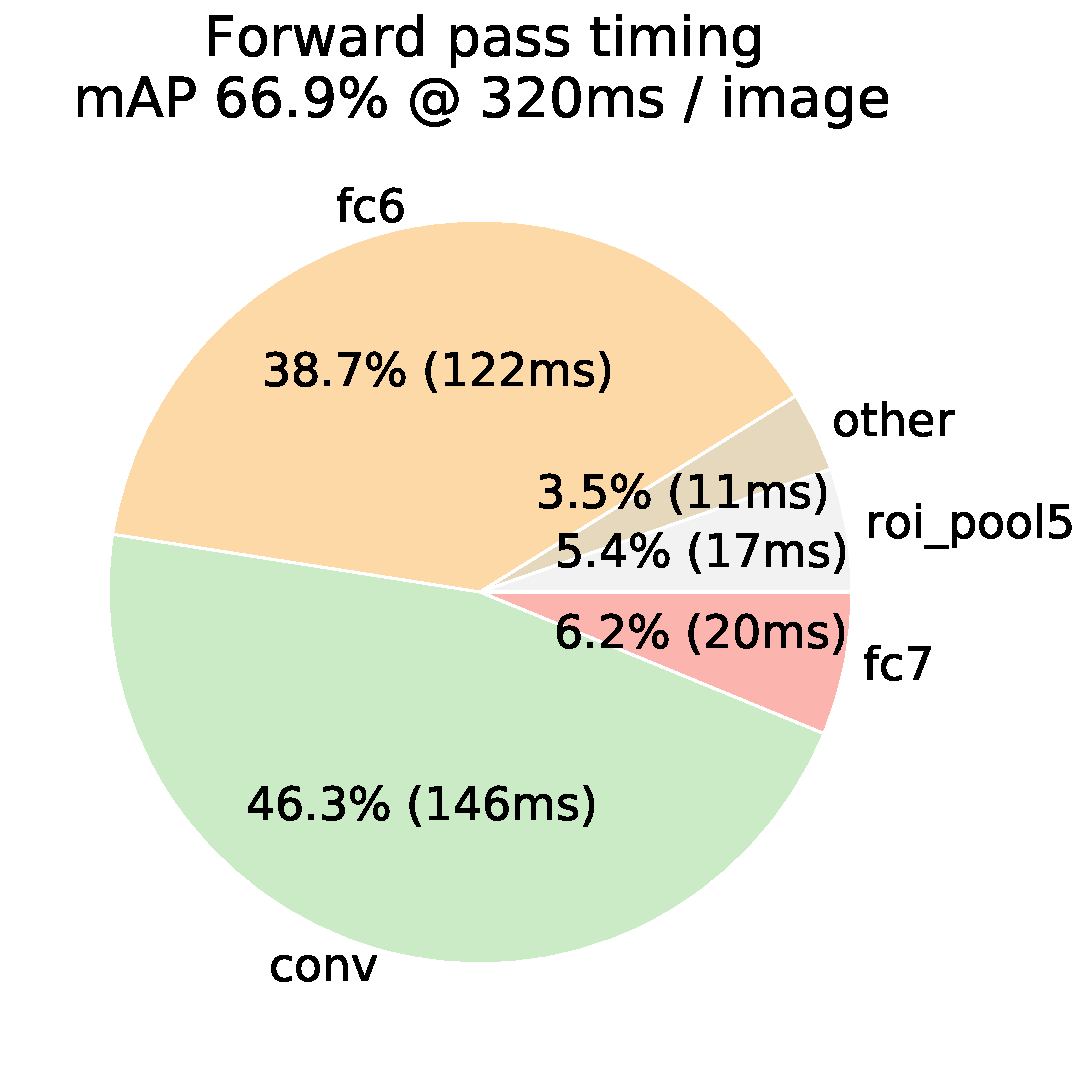
\includegraphics[width=0.49\linewidth,trim=3em 2em 0 0, clip]{figs/layer_timing.pdf}
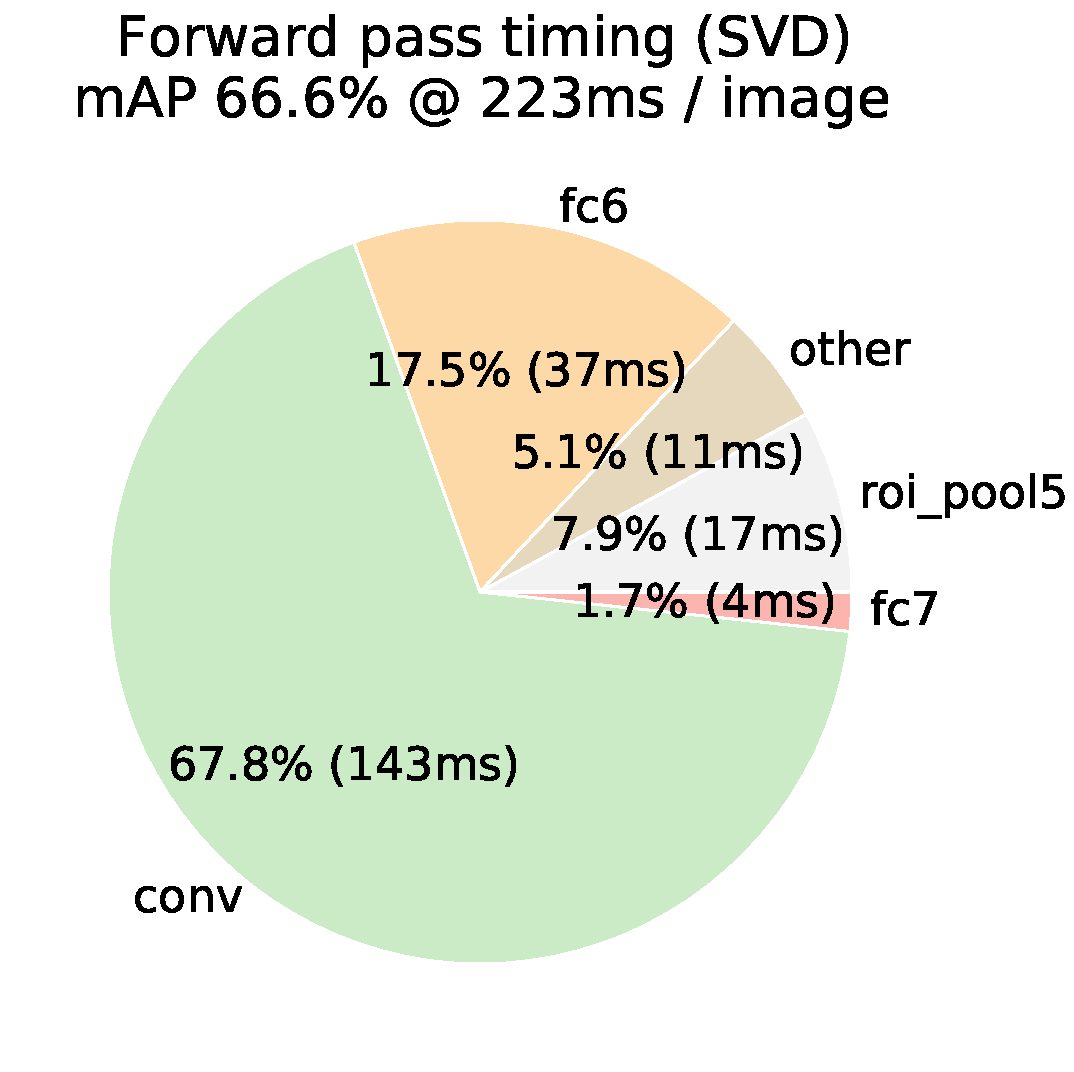
\includegraphics[width=0.49\linewidth,trim=3em 2em 0 0, clip]{figs/layer_timing_svd.pdf}
%\vspace{-1em}
\caption{Timing for \vggsixteen before and after truncated SVD.
Before SVD, fully connected layers fc6 and fc7 take 45\% of the time.}
\figlabel{timing}
\end{figure}

%\begin{table}[h!]
%\begin{center}
%\setlength{\tabcolsep}{6pt}
%\renewcommand{\arraystretch}{1.1}
%\small
%\begin{tabular}{l|rr|rr|rr}
%  & \multicolumn{2}{c|}{\Sm} & \multicolumn{2}{c|}{\Med} & \multicolumn{2}{c}{\Lg} \\
%\hline
%Trunc. SVD? &  & \checkmark &  & \checkmark & & \checkmark \\
%s / image & 0.10 & 0.06 & 0.15 & 0.08 & 0.32 & 0.22 \\
%VOC07 mAP & 57.1 & 56.5 & 59.2 & 58.7 & 66.9 & 66.6
%\end{tabular}
%\end{center}
%\caption{Effects of truncated SVD on test speed and mAP.}
%\tablelabel{svd}
%\end{table}
%
%\tableref{svd} shows results for all three models using the top 1024 and 256 singular values for layers fc6 and fc7, respectively.
%Even though the compression factor increases from \Sm to \Lg, the loss in mAP decreases.

\subsection{Which layers to fine-tune?}
For the less deep networks considered in the SPPnet paper \cite{he2014spp}, fine-tuning only the fully connected layers appeared to be sufficient for good accuracy.
We hypothesized that this result would not hold for very deep networks.
To validate that fine-tuning the conv layers is important for \vggsixteen, we use Fast R-CNN to fine-tune, but \emph{freeze} the thirteen conv layers so that only the fully connected layers learn.
This ablation emulates single-scale SPPnet training and \emph{decreases mAP from 66.9\% to 61.4\%} (\tableref{whichlayers}).
This experiment verifies our hypothesis: training through the \roi pooling layer is important for very deep nets.

\begin{table}[h!]
\begin{center}
\setlength{\tabcolsep}{3pt}
\renewcommand{\arraystretch}{1.1}
\small
\begin{tabular}{l|rrr|r}
  & \multicolumn{3}{c|}{layers that are fine-tuned in model \Lg} & SPPnet \Lg \\
  & $\ge$ fc6 & $\ge$ conv3\_1 & $\ge$ conv2\_1 & $\ge$ fc6 \\
\hline
VOC07 mAP & 61.4 & 66.9 & \bf{67.2} & 63.1 \\
test rate (s/im) & \bf{0.32} & \bf{0.32} & \bf{0.32} & 2.3 \\
\end{tabular}
\end{center}
\caption{Effect of restricting which layers are fine-tuned for \vggsixteen.
Fine-tuning $\ge$ fc6 emulates the SPPnet training algorithm \cite{he2014spp}, but using a single scale.
SPPnet \Lg results were obtained using five scales, at a significant (7\X) speed cost.}
\tablelabel{whichlayers}
\vspace{-0.5em}
\end{table}

Does this mean that \emph{all} conv layers should be fine-tuned? In short, \emph{no}.
In the smaller networks (\Sm and \Med) we find that conv1 is generic and task independent (a well-known fact \cite{krizhevsky2012imagenet}).
Allowing conv1 to learn, or not, has no meaningful effect on mAP.
For \vggsixteen, we found it only necessary to update layers from conv3\_1 and up (9 of the 13 conv layers).
This observation is pragmatic: (1) updating from conv2\_1 slows training by 1.3\X (12.5 vs. 9.5 hours) compared to learning from conv3\_1;
and (2) updating from conv1\_1 over-runs GPU memory.
The difference in mAP when learning from conv2\_1 up was only $+0.3$ points (\tableref{whichlayers}, last column).
All Fast R-CNN results in this paper using \vggsixteen fine-tune layers conv3\_1 and up; all experiments with models \Sm and \Med fine-tune layers conv2 and up.

\begin{table*}[t!]
\begin{center}
\setlength{\tabcolsep}{5pt}
\renewcommand{\arraystretch}{1.1}
\small
\begin{tabular}{l|rrrr|rrrr|rrrr}
  & \multicolumn{4}{c|}{\Sm} & \multicolumn{4}{c|}{\Med} & \multicolumn{4}{c}{\Lg}  \\
\hline
multi-task training? &
&
\checkmark &
&
\checkmark &
&
\checkmark &
&
\checkmark &
&
\checkmark &
&
\checkmark
\\
stage-wise training? &
 &
 &
\checkmark &
&
 &
 &
\checkmark &
&
 &
 &
\checkmark &
\\
test-time bbox reg? & & & \checkmark & \checkmark & & & \checkmark & \checkmark & & & \checkmark & \checkmark \\
VOC07 mAP & 52.2 & 53.3 & 54.6 & \bf{57.1} & 54.7 & 55.5 & 56.6 & \bf{59.2} & 62.6 & 63.4 & 64.0 & \bf{66.9} \\
\end{tabular}
\end{center}
\caption{Multi-task training (forth column per group) improves mAP over piecewise training (third column per group).}
\tablelabel{multitask}
\vspace{-0.5em}
\end{table*}

\section{Design evaluation}

We conducted experiments to understand how Fast R-CNN compares to R-CNN and SPPnet, as well as to evaluate design decisions.
Following best practices, we performed these experiments on the PASCAL VOC07 dataset.
%Based on those results, we train and test a couple of models on VOC12.

\subsection{Does multi-task training help?}
\seclabel{multitask}
Multi-task training is convenient because it avoids managing a pipeline of sequentially-trained tasks.
But it also has the potential to improve results because the tasks influence each other through a shared representation (the ConvNet) \cite{caruana1997multitask}.
Does multi-task training improve object detection accuracy in Fast R-CNN?

To test this question, we train baseline networks that use only the classification loss, $L_\textrm{cls}$, in \eqref{loss} (\ie, setting $\lambda = 0$).
These baselines are printed for models \Sm, \Med, and \Lg in the first column of each group in \tableref{multitask}.
Note that these models \emph{do not} have bounding-box regressors.
Next (second column per group), we take networks that were trained with the multi-task loss (\eqref{loss}, $\lambda = 1$), but we \emph{disable} bounding-box regression at test time.
This isolates the networks' classification accuracy and allows an apples-to-apples comparison with the baseline networks.
%(Results with bounding-box regression are shown in the third column, per group, to illustrate its effect.)

Across all three networks we observe that multi-task training improves pure classification accuracy relative to training for classification alone.
The improvement ranges from $+0.8$ to $+1.1$ mAP points, showing a consistent positive effect from multi-task learning.

Finally, we take the baseline models (trained with only the classification loss), tack on the bounding-box regression layer, and train them with $L_{loc}$ while keeping all other network parameters frozen.
The third column in each group shows the results of this \emph{stage-wise} training scheme: mAP improves over column one, but stage-wise training underperforms multi-task training (forth column per group).

\subsection{Scale invariance: to brute force or finesse?}
\seclabel{scale}
We compare two strategies for achieving scale-invariant object detection: brute-force learning (single scale) and image pyramids (multi-scale).
In either case, we define the scale $s$ of an image to be the length of its \emph{shortest} side.

All single-scale experiments use $s = 600$ pixels;
$s$ may be less than $600$ for some images as we cap the longest image side at $1000$ pixels and maintain the image's aspect ratio.
These values were selected so that \vggsixteen fits in GPU memory during fine-tuning.
The smaller models are not memory bound and can benefit from larger values of $s$; however, optimizing $s$ for each model is not our main concern.
We note that PASCAL images are $384 \times 473$ pixels on average and thus the single-scale setting typically upsamples images by a factor of 1.6.
The average effective stride at the \roi pooling layer is thus $\approx 10$ pixels.

In the multi-scale setting, we use the same five scales specified in \cite{he2014spp} ($s \in \{480, 576, 688, 864, 1200\}$) to facilitate comparison with SPPnet.
However, we cap the longest side at $2000$ pixels to avoid exceeding GPU memory.

\begin{table}[h!]
\begin{center}
\setlength{\tabcolsep}{4.7pt}
\renewcommand{\arraystretch}{1.1}
\small
\begin{tabular}{l|rr|rr|rr|r}
 & \multicolumn{2}{c|}{SPPnet \ZF}  & \multicolumn{2}{c|}{\Sm} & \multicolumn{2}{c|}{\Med} & \Lg \\
\hline
scales & 1 & 5 & 1 & 5 & 1 & 5 & 1 \\
test rate (s/im) & 0.14 & 0.38 & \bf{0.10} & 0.39 & 0.15 & 0.64 & 0.32 \\
VOC07 mAP & 58.0 & 59.2 & 57.1 & 58.4 & 59.2 & 60.7 & \bf{66.9}
\end{tabular}
\end{center}
\caption{Multi-scale vs. single scale.
SPPnet \ZF (similar to model \Sm) results are from \cite{he2014spp}.
Larger networks with a single-scale offer the best speed / accuracy tradeoff.
(\Lg cannot use multi-scale in our implementation due to GPU memory constraints.)
}
\tablelabel{scales}
\vspace{-0.5em}
\end{table}

\tableref{scales} shows models \Sm and \Med when trained and tested with either one or five scales.
Perhaps the most surprising result in \cite{he2014spp} was that single-scale detection performs almost as well as multi-scale detection.
Our findings confirm their result: deep ConvNets are adept at directly learning scale invariance.
The multi-scale approach offers only a small increase in mAP at a large cost in compute time (\tableref{scales}).
In the case of \vggsixteen (model \Lg), we are limited to using a single scale by implementation details. Yet it achieves a mAP of 66.9\%, which is slightly higher than the 66.0\% reported for R-CNN \cite{rcnn-pami}, even though R-CNN uses ``infinite'' scales in the sense that each proposal is warped to a canonical size.

Since single-scale processing offers the best tradeoff between speed and accuracy, especially for very deep models, all experiments outside of this sub-section use single-scale training and testing with $s = 600$ pixels.

\subsection{Do we need more training data?}
\seclabel{moredata}
A good object detector should improve when supplied with more training data.
Zhu \etal \cite{devaMoreData} found that DPM \cite{lsvm-pami} mAP saturates after only a few hundred to thousand training examples.
Here we augment the VOC07 trainval set with the VOC12 trainval set, roughly tripling the number of images to 16.5k, to evaluate Fast R-CNN.
%\cite{agrawal2014analyzing}.
Enlarging the training set improves mAP on VOC07 test from 66.9\% to 70.0\% (\tableref{voc2007}).
When training on this dataset we use 60k mini-batch iterations instead of 40k.

We perform similar experiments for VOC10 and 2012, for which we construct a dataset of 21.5k images from the union of VOC07 trainval, test, and VOC12 trainval.
When training on this dataset, we use 100k SGD iterations and lower the learning rate by $0.1\times$ each 40k iterations (instead of each 30k).
For VOC10 and 2012, mAP improves from 66.1\% to 68.8\% and from 65.7\% to 68.4\%, respectively.
%Fast R-CNN accuracy should improve if more training data become available.

\subsection{Do SVMs outperform softmax?}
Fast R-CNN uses the softmax classifier learnt during fine-tuning instead of training one-vs-rest linear SVMs post-hoc, as was done in R-CNN and SPPnet.
To understand the impact of this choice, we implemented post-hoc SVM training with hard negative mining in Fast R-CNN.
We use the same training algorithm and hyper-parameters as in R-CNN.
\begin{table}[h!]
\begin{center}
\setlength{\tabcolsep}{6pt}
\renewcommand{\arraystretch}{1.1}
\small
\begin{tabular}{l|l|r|r|r}
  method & classifier & \Sm & \Med & \Lg \\
\hline
R-CNN \cite{girshick2014rcnn,rcnn-pami} & SVM & \bf{58.5} & \bf{60.2} & 66.0 \\
\hline
FRCN [ours] & SVM & 56.3 & 58.7 & 66.8 \\
FRCN [ours] & softmax & 57.1 & 59.2 & \bf{66.9} \\
\end{tabular}
\end{center}
\caption{Fast R-CNN with softmax vs. SVM (VOC07 mAP).}
\tablelabel{svm}
\vspace{-0.5em}
\end{table}

\tableref{svm} shows softmax slightly outperforming SVM for all three networks, by $+0.1$ to $+0.8$ mAP points.
This effect is small, but it demonstrates that ``one-shot'' fine-tuning is sufficient compared to previous multi-stage training approaches.
We note that softmax, unlike one-vs-rest SVMs, introduces competition between classes when scoring a \roi.

\subsection{Are more proposals always better?}

%Fast R-CNN enables researchers to test ideas that would have been prohibitively slow in the past.
%For example, we can study the behavior of Fast R-CNN when using a large number of object proposals.

There are (broadly) two types of object detectors: those that use a \emph{sparse} set of object proposals (\eg, selective search \cite{UijlingsIJCV2013}) and those that use a \emph{dense} set (\eg, DPM \cite{lsvm-pami}).
Classifying sparse proposals is a type of \emph{cascade} \cite{Viola01} in which the proposal mechanism first rejects a vast number of candidates leaving the classifier with a small set to evaluate.
This cascade improves detection accuracy when applied to DPM detections \cite{UijlingsIJCV2013}.
We find evidence that the proposal-classifier cascade also improves Fast R-CNN accuracy.

%\paragraph{More sparse proposals.}
Using selective search's \emph{quality mode}, we sweep from 1k to 10k proposals per image, each time \emph{re-training} and \emph{re-testing} model \Med.
If proposals serve a purely computational role, increasing the number of proposals per image should not harm mAP.
\begin{figure}[h!]
\centering
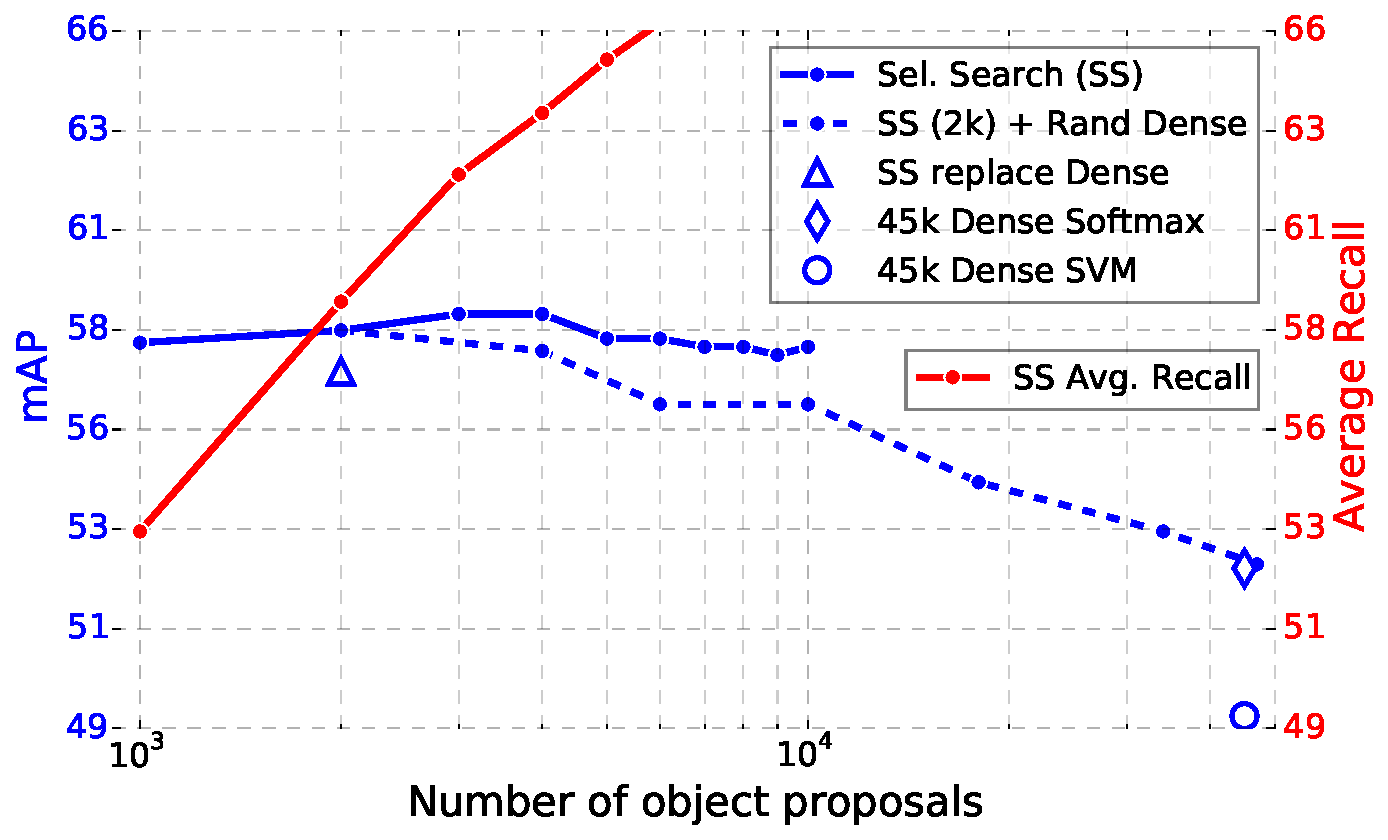
\includegraphics[width=1\linewidth,trim=0em 0em 0 0, clip]{figs/proposals.pdf}
%\vspace{-1em}
\caption{VOC07 test mAP and AR for various proposal schemes.}
\figlabel{proposals}
\end{figure}

We find that  mAP rises and then falls slightly as the proposal count increases (\figref{proposals}, solid blue line).
This experiment shows that swamping the deep classifier with more proposals does not help, and even slightly hurts, accuracy.

This result is difficult to predict without actually running the experiment.
The state-of-the-art for measuring object proposal quality is Average Recall (AR) \cite{Hosang15proposals}.
AR correlates well with mAP for several proposal methods using R-CNN, \emph{when using a fixed number of proposals per image}.
\figref{proposals} shows that AR (solid red line) does not correlate well with mAP as the number of proposals per image is varied.
AR must be used with care; higher AR due to more proposals does not imply that mAP will increase.
Fortunately, training and testing with model \Med takes less than 2.5 hours.
Fast R-CNN thus enables efficient, direct evaluation of object proposal mAP, which is preferable to proxy metrics.


%\paragraph{Dense proposals.}
We also investigate Fast R-CNN when using \emph{densely} generated boxes (over scale, position, and aspect ratio), at a rate of about 45k boxes / image.
This dense set is rich enough that when each selective search box is replaced by its closest (in IoU) dense box, mAP drops only 1 point (to 57.7\%, \figref{proposals}, blue triangle).

The statistics of the dense boxes differ from those of selective search boxes.
Starting with 2k selective search boxes, we test mAP when \emph{adding} a random sample of $1000 \times \{2,4,6,8,10,32,45\}$ dense boxes.
For each experiment we re-train and re-test model \Med.
When these dense boxes are added, mAP falls more strongly than when adding more selective search boxes, eventually reaching 53.0\%.

We also train and test Fast R-CNN using \emph{only} dense boxes (45k / image).
This setting yields a mAP of 52.9\% (blue diamond).
Finally, we check if SVMs with hard negative mining are needed to cope with the dense box distribution.
SVMs do even worse: 49.3\% (blue circle).

%\paragraph{Dense vs. sparse.}
%Sparse object proposal methods are currently the speed bottleneck in Fast R-CNN.
%%Selective search takes 2s / image and EdgeBoxes takes 0.2s / image.
%Replacing them with a dense set of ``sliding windows'' is attractive, since it is essentially free.
%Yet, these experiments provide the first evidence that sparse proposals do indeed ``improve detection quality by reducing spurious false positives'' \cite{Hosang15proposals}.

\subsection{Preliminary MS COCO results}
We applied Fast R-CNN (with \vggsixteen) to the MS COCO dataset \cite{coco} to establish a preliminary baseline.
We trained on the 80k image training set for 240k iterations and evaluated on the ``test-dev'' set using the evaluation server.
The PASCAL-style mAP is 35.9\%; the new COCO-style AP, which also averages over IoU thresholds, is 19.7\%.

\label{sec:conclusion}
We introduce a novel neural network architecture, the Synchronized Spectral CNN (SyncSpecCNN), for semantic annotation on 3D shape graphs. To share coefficients and conduct multi-scale analysis in different parts of a single shape graph, we introduce a spectral parametrization of dilated convolutional kernels. To allow parameter sharing across related but different shapes that may be represented by very different graphs, we introduce a spectral transformer network to synchronize different spectral domains. The effectiveness of different components in our network is validated through extensive experiments. Jointly these contributions lead to state-of-the-art performance on various semantic annotation tasks including 3D shape part segmentation and 3D keypoint prediction.

\paragraph{Acknowledgements.}
I thank Kaiming He, Larry Zitnick, and Piotr Doll{\'a}r for helpful discussions and encouragement.

{\small
\bibliographystyle{ieee}
\bibliography{main}
}

\end{document}
